\chapter{Experiments and Evaluation}\label{experiment}

\section{Simulation of Flocking Models}

We first show the influence of $\sigma$ and $\beta$ in (\ref{eq:proposed_ui}) to the convergence of the flock by Fig.\ref{fig:sigma_beta}, where the averaged $\psi_{scal}$ (\ref{eq:psi_scal}) of twenty simulation results are illustrated with three cases. The more $\psi_{scal}$ gets close to 1, the more convergent and aligned the flock is. As shown in the figure that the choice of $\sigma$ has little impact on the convergence rate compared with $\beta$. When $\beta\leq\frac{1}{2}$, the convergence of the whole flock is unconditional which is coincident with our assumption in Ch.~\ref{control_law}. Without explicit statement, all the following simulations use $\sigma=1$ and $\beta=0.25$. We then compute the averaged results of $\psi_{scal}$ and relative distance from twenty simulations as illustrated in Fig.\ref{fig:multiple_agent}. We show that the number of total agents in the flock does not influence the characteristics of cohesion, separation and alignment.

\begin{figure}[H]
  \centering
  \subfigure[Average $\psi_{scal}$ of multiple agents with fixed $\sigma, \beta$]{\label{fig:multiple}\includegraphics[width=0.49\textwidth]{figure/chapter_5/multiple.png}}
  \subfigure[Average distance of multiple agents with fixed $\sigma, \beta$]{\label{fig:distance}\includegraphics[width=0.49\textwidth]{figure/chapter_5/distance.png}}
  \caption{Average $\psi_{scal}$ and relative distance of multiple agents with fixed $\sigma=1$ and $\beta=0.25$. Their initial velocity are all randomized and nonzero.}\label{fig:multiple_agent}
\end{figure}

\begin{figure}[H]
  \centering
  \subfigure[Case 1: $\sigma<1$ with $\sigma=0.5$]{\label{fig:sigma0_5}\includegraphics[width=0.49\textwidth]{figure/chapter_5/sigma0_5.png}}
  \subfigure[Case 2: $\sigma=1$]{\label{fig:sigma1}\includegraphics[width=0.49\textwidth]{figure/chapter_5/sigma1.png}}
  \quad
  \subfigure[Case 3: $\sigma>1$ with $\sigma=1.5$]{\label{fig:sigma1_5}\includegraphics[width=0.49\textwidth]{figure/chapter_5/sigma1_5.png}}
  \caption{Averaged $\psi_{scal}$ of twenty simulations of two agents w.r.t various $\sigma, \beta$. Their initial velocities are all randomized and nonzero.}\label{fig:sigma_beta}
\end{figure}

We compare our proposed flocking model with the ones in~\cite{Vicsek1995,CuckerSmale2007,CuckerDong2010} in Ch.~\ref{flocking} with 2, 3 and 4 agents respectively. The initial position are illustrated in Fig.\ref{fig:simulate_flocking} where the initial velocities are randomized and normalized. The positions of individual agents during the whole simulation are illustrated in Fig.\ref{fig:N_pos} for reference. As illustrated in Fig.\ref{fig:N_scal}, we show that our proposed model converge as fast as those in~\cite{Vicsek1995,CuckerSmale2007,CuckerDong2010}. Especially, we show that the relative distance between neighboring agents in our proposed model is strictly bounded by the interval $(d_0^{\frac{1}{2}}, d_0^{\frac{1}{2}})$. Suppose certain minimum safety distance exists, such as $d_{safe}=0.8$ in Fig.\ref{fig:N3_dis}, our proposed model could successfully avoided collision with neighboring agents.

\begin{figure}[H]
  \centering
  \subfigure[Two agents in a shape of straight line]{\label{fig:2_agents}\includegraphics[width=0.32\textwidth]{figure/chapter_5/2_agent.png}}
  \subfigure[Three agents in a shape of equilateral triangle]{\label{fig:2_agents}\includegraphics[width=0.32\textwidth]{figure/chapter_5/3_agent.png}}
  \subfigure[Four agents in a shape of diamond]{\label{fig:2_agents}\includegraphics[width=0.32\textwidth]{figure/chapter_5/4_agent.png}}
  \caption{Initial position settings of multi-agent flocking simulations in MATLAB.}\label{fig:simulate_flocking}
\end{figure}

\begin{figure}[H]
  \centering
  \subfigure[$N=2$ agents]{\label{fig:N2_scal}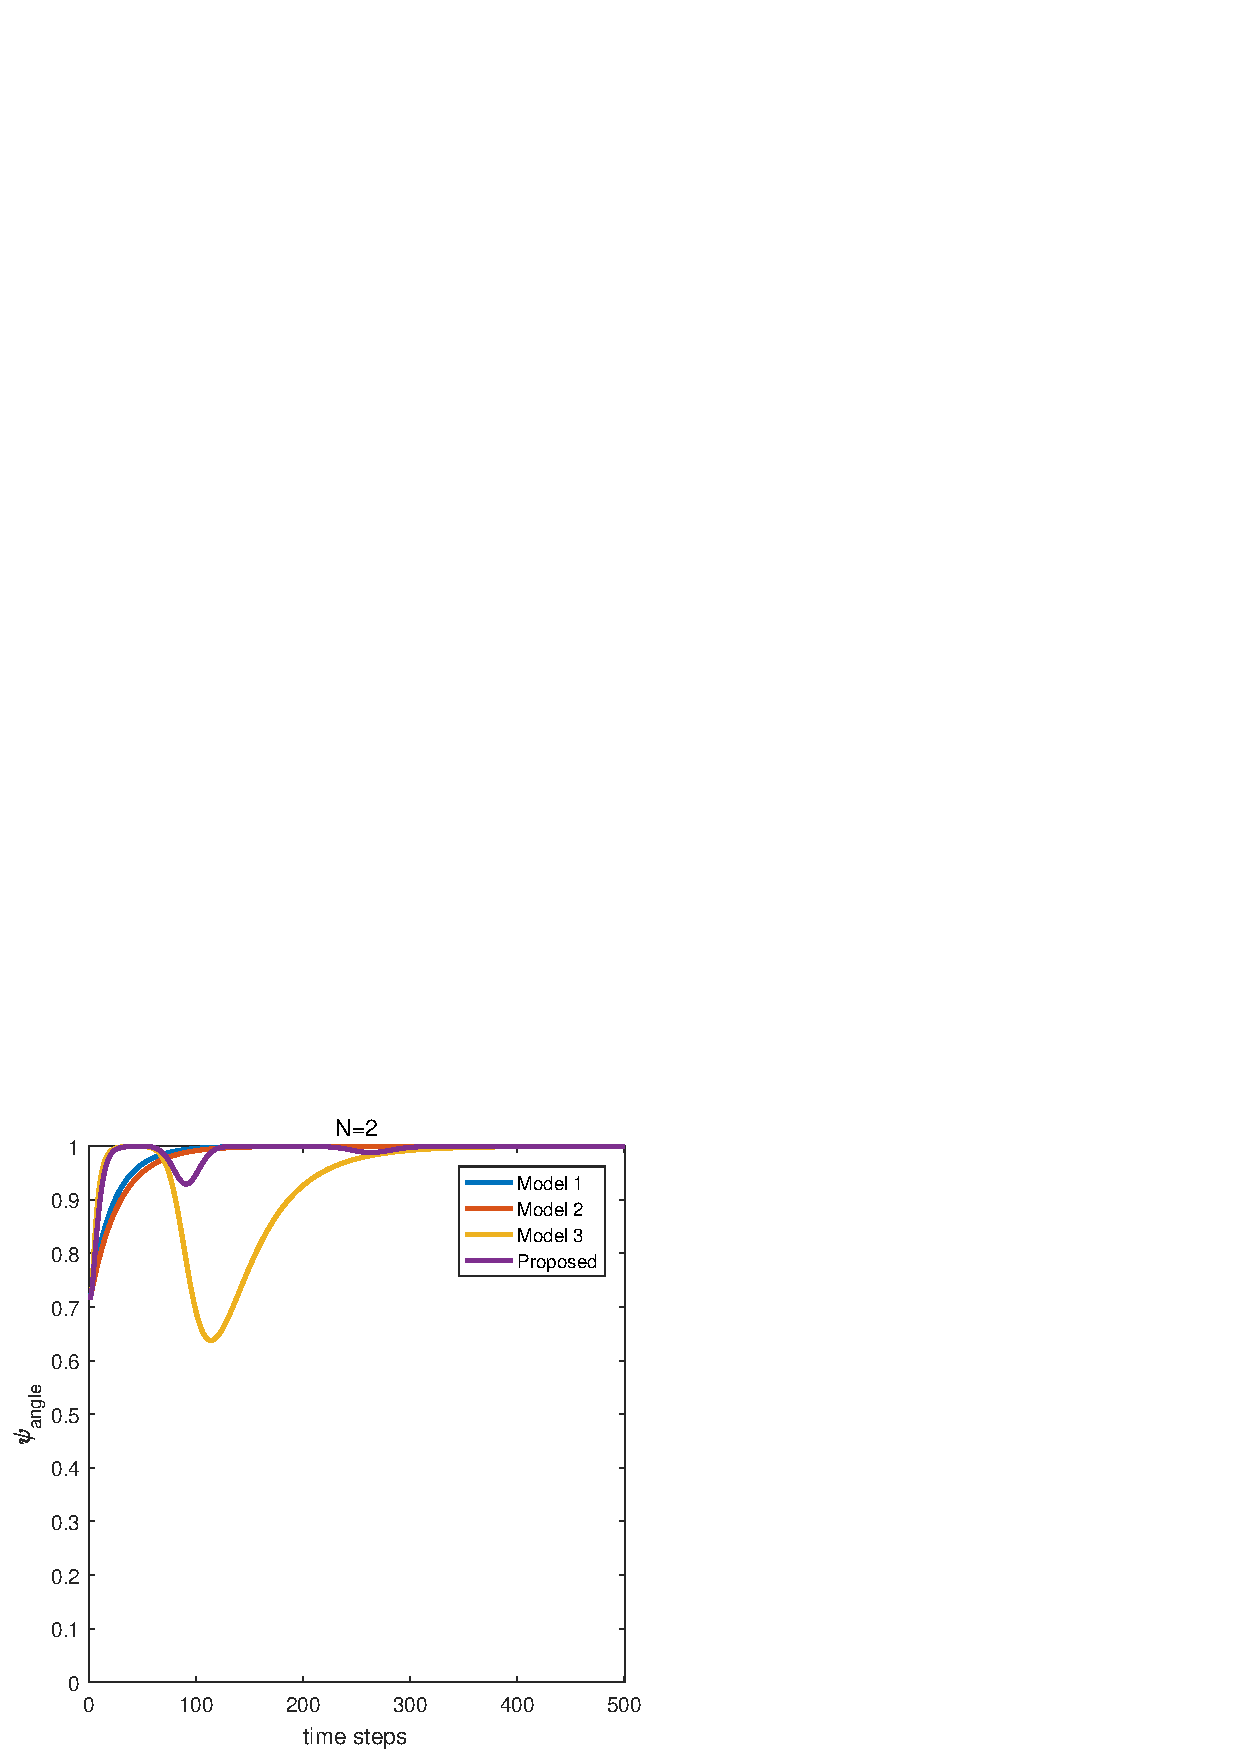
\includegraphics[width=0.49\textwidth]{figure/chapter_5/N2_scal.png}}
  \subfigure[$N=3$ agents]{\label{fig:N3_scal}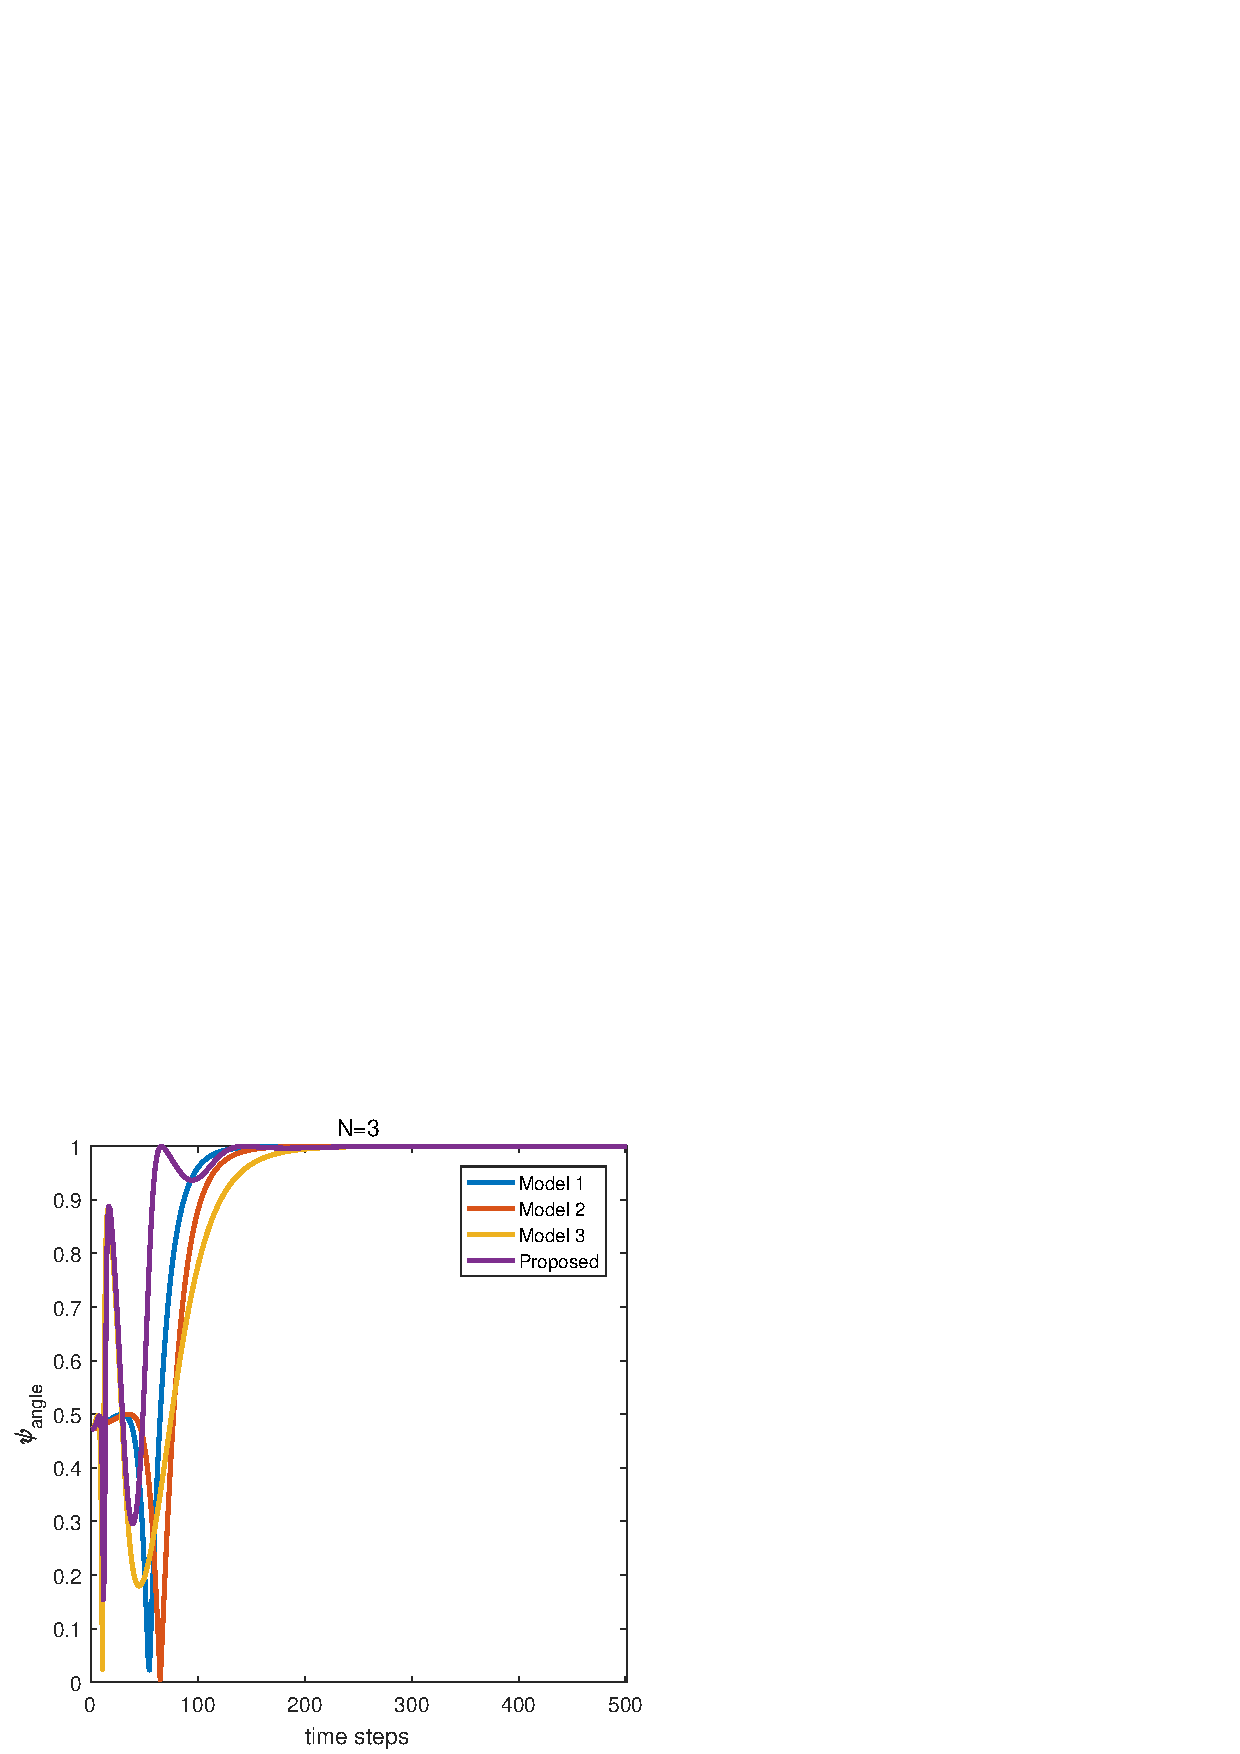
\includegraphics[width=0.49\textwidth]{figure/chapter_5/N3_scal.png}}
  \quad
  \subfigure[$N=4$ agents]{\label{fig:N4_scal}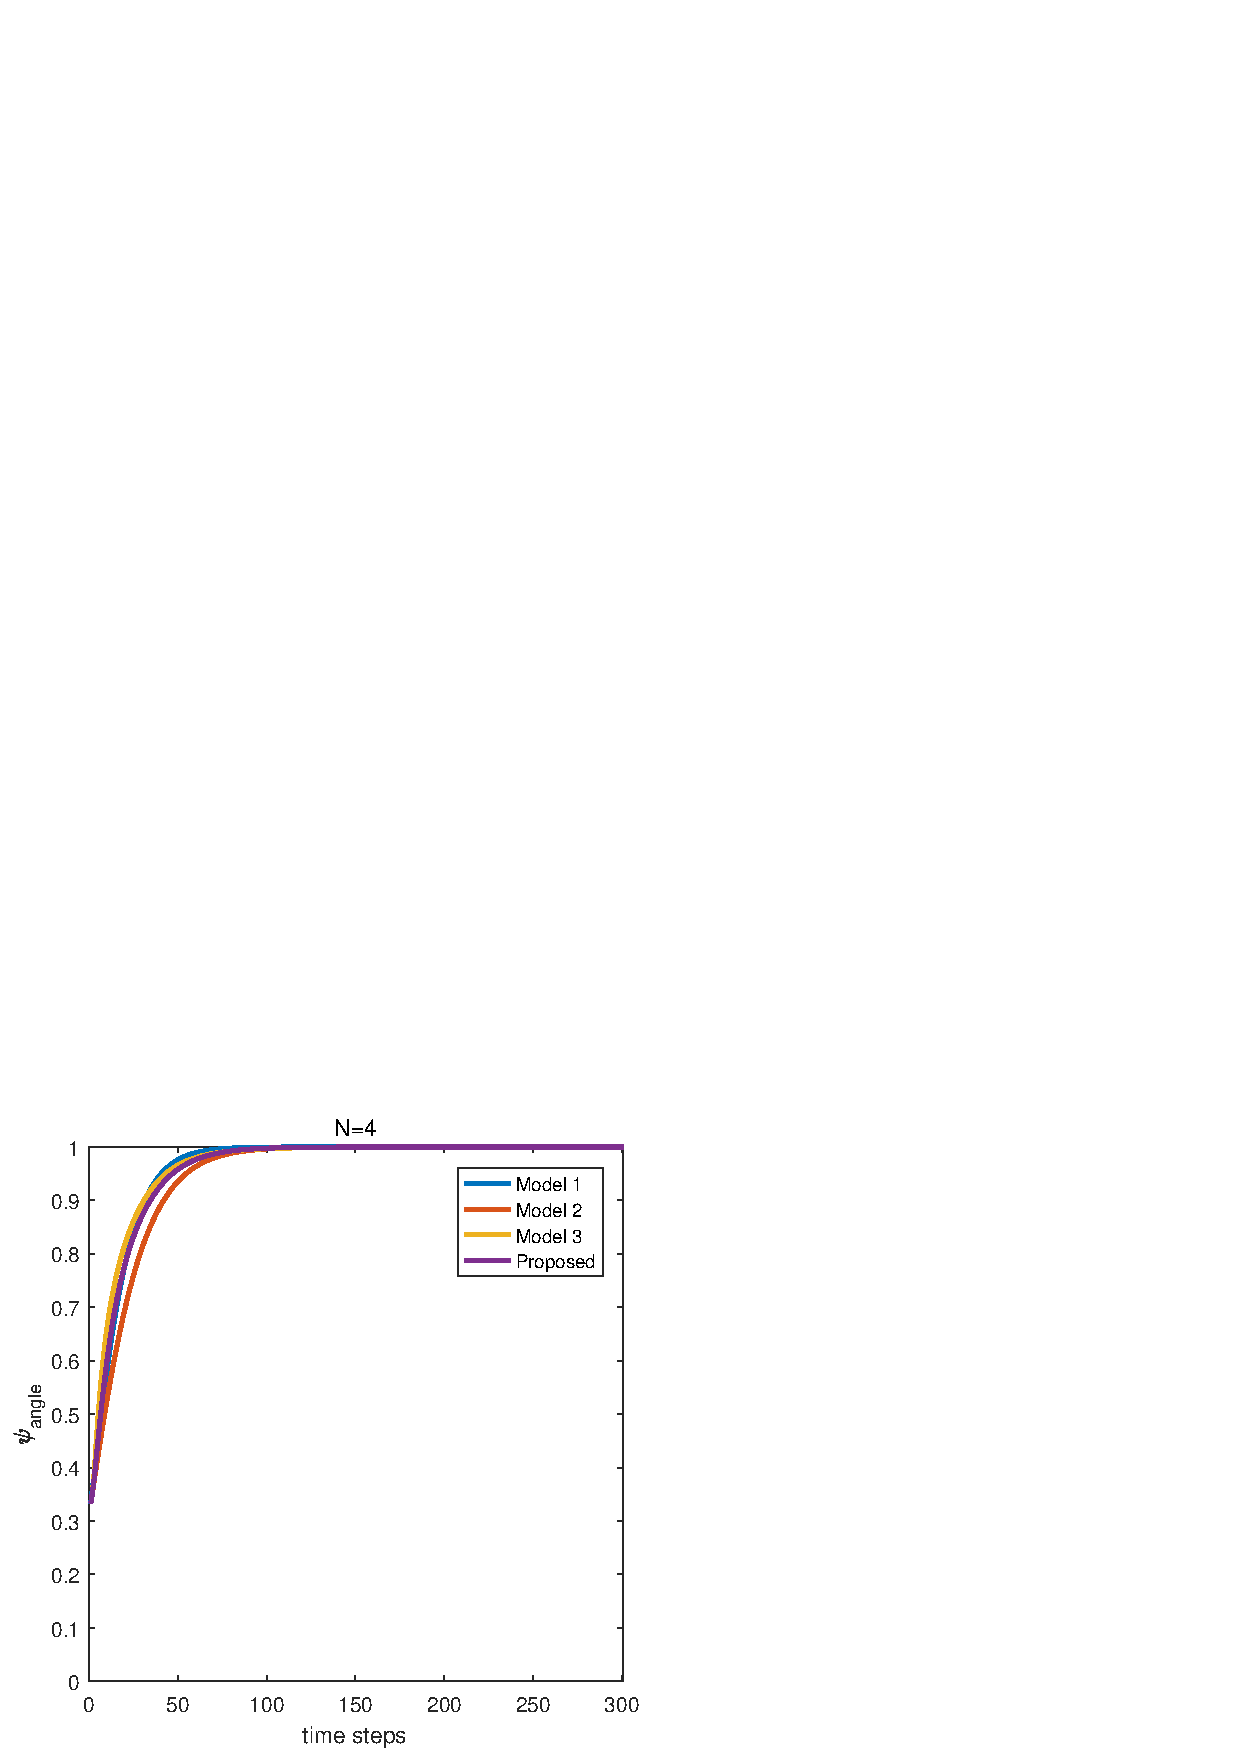
\includegraphics[width=0.49\textwidth]{figure/chapter_5/N4_scal.png}}
  \caption{Convergence descriptor $\psi_{scal}$ of model 1 (\cite{Vicsek1995}), 2 (\cite{CuckerSmale2007}), 3 (\cite{CuckerDong2010}) and our proposed one.}\label{fig:N_scal}
\end{figure}

\begin{figure}[H]
  \centering
  \subfigure[$N=2$ agents.]{\label{fig:N2_dis}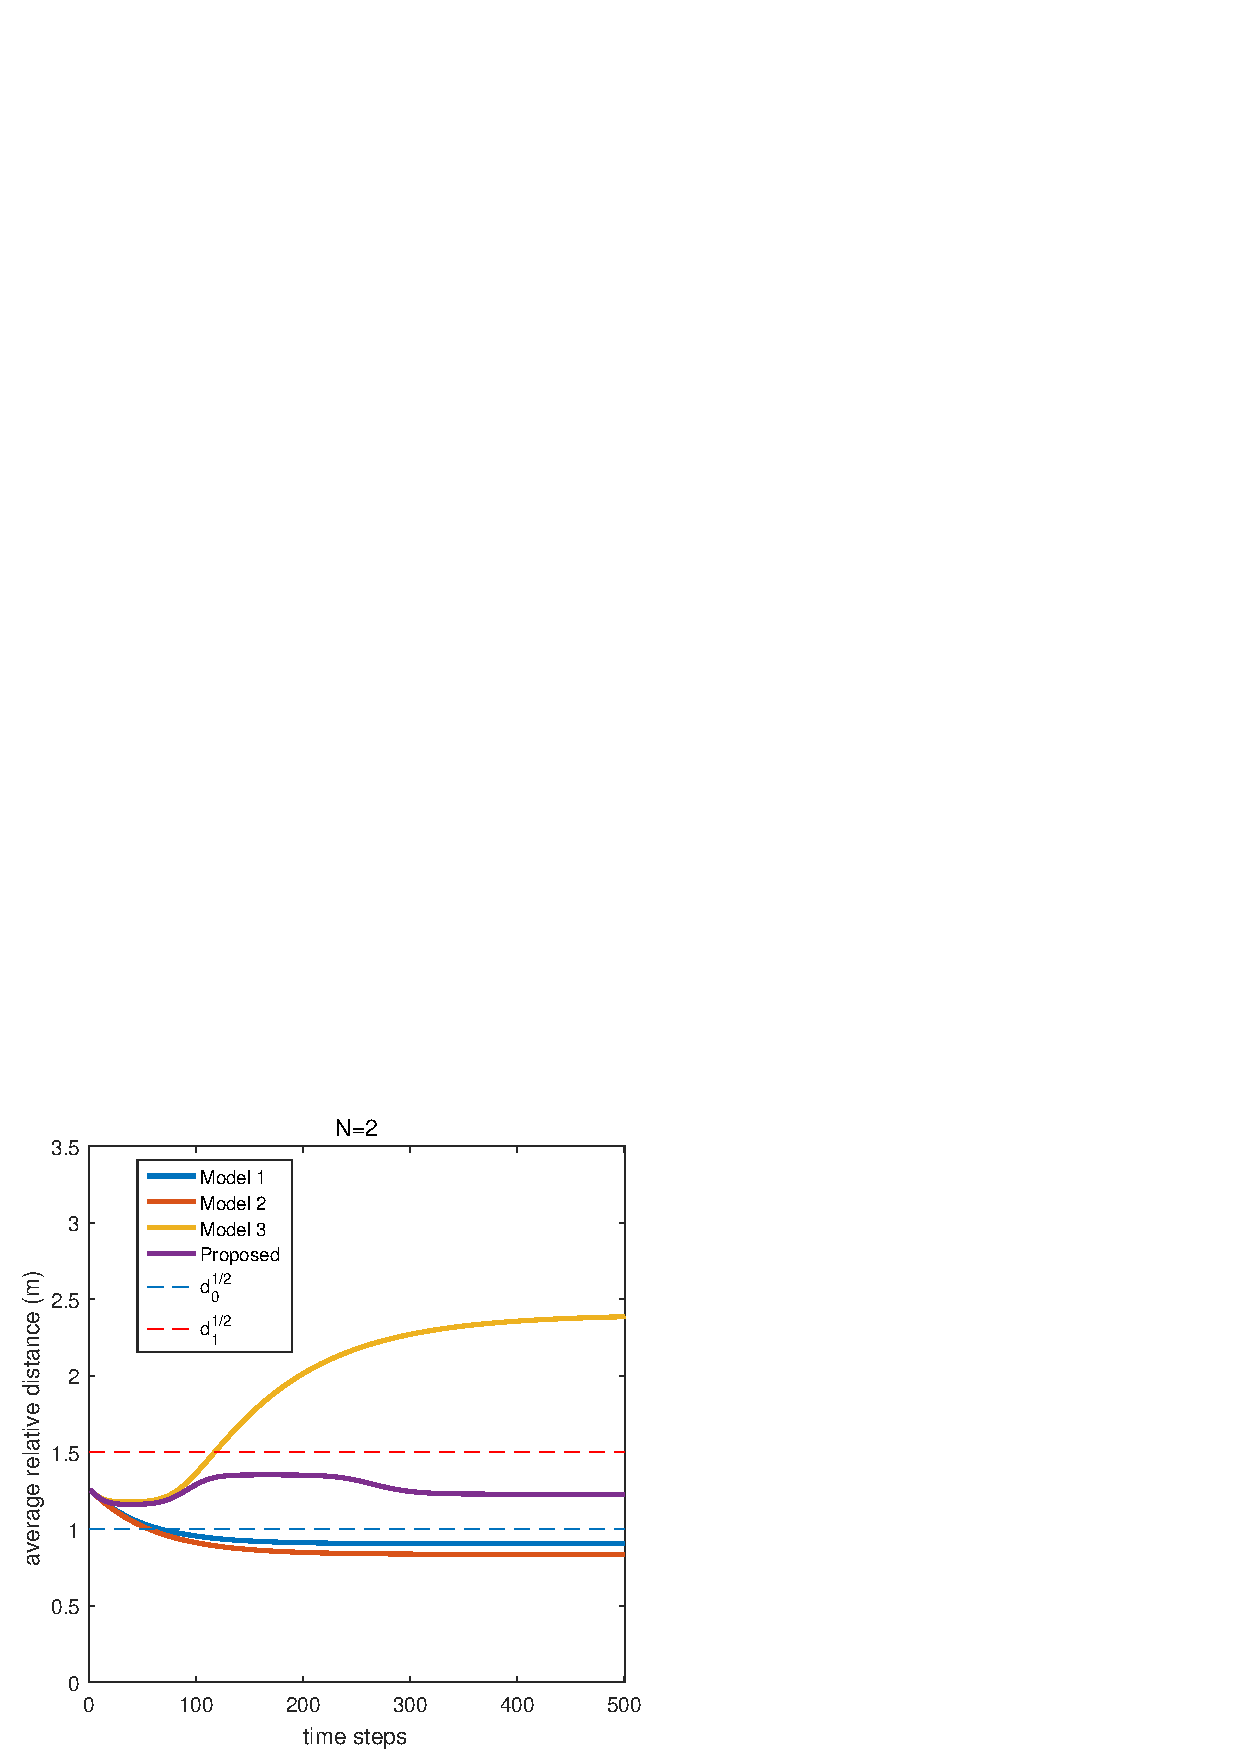
\includegraphics[width=0.49\textwidth]{figure/chapter_5/N2_dis.png}}
  \subfigure[$N=3$ agents.]{\label{fig:N3_dis}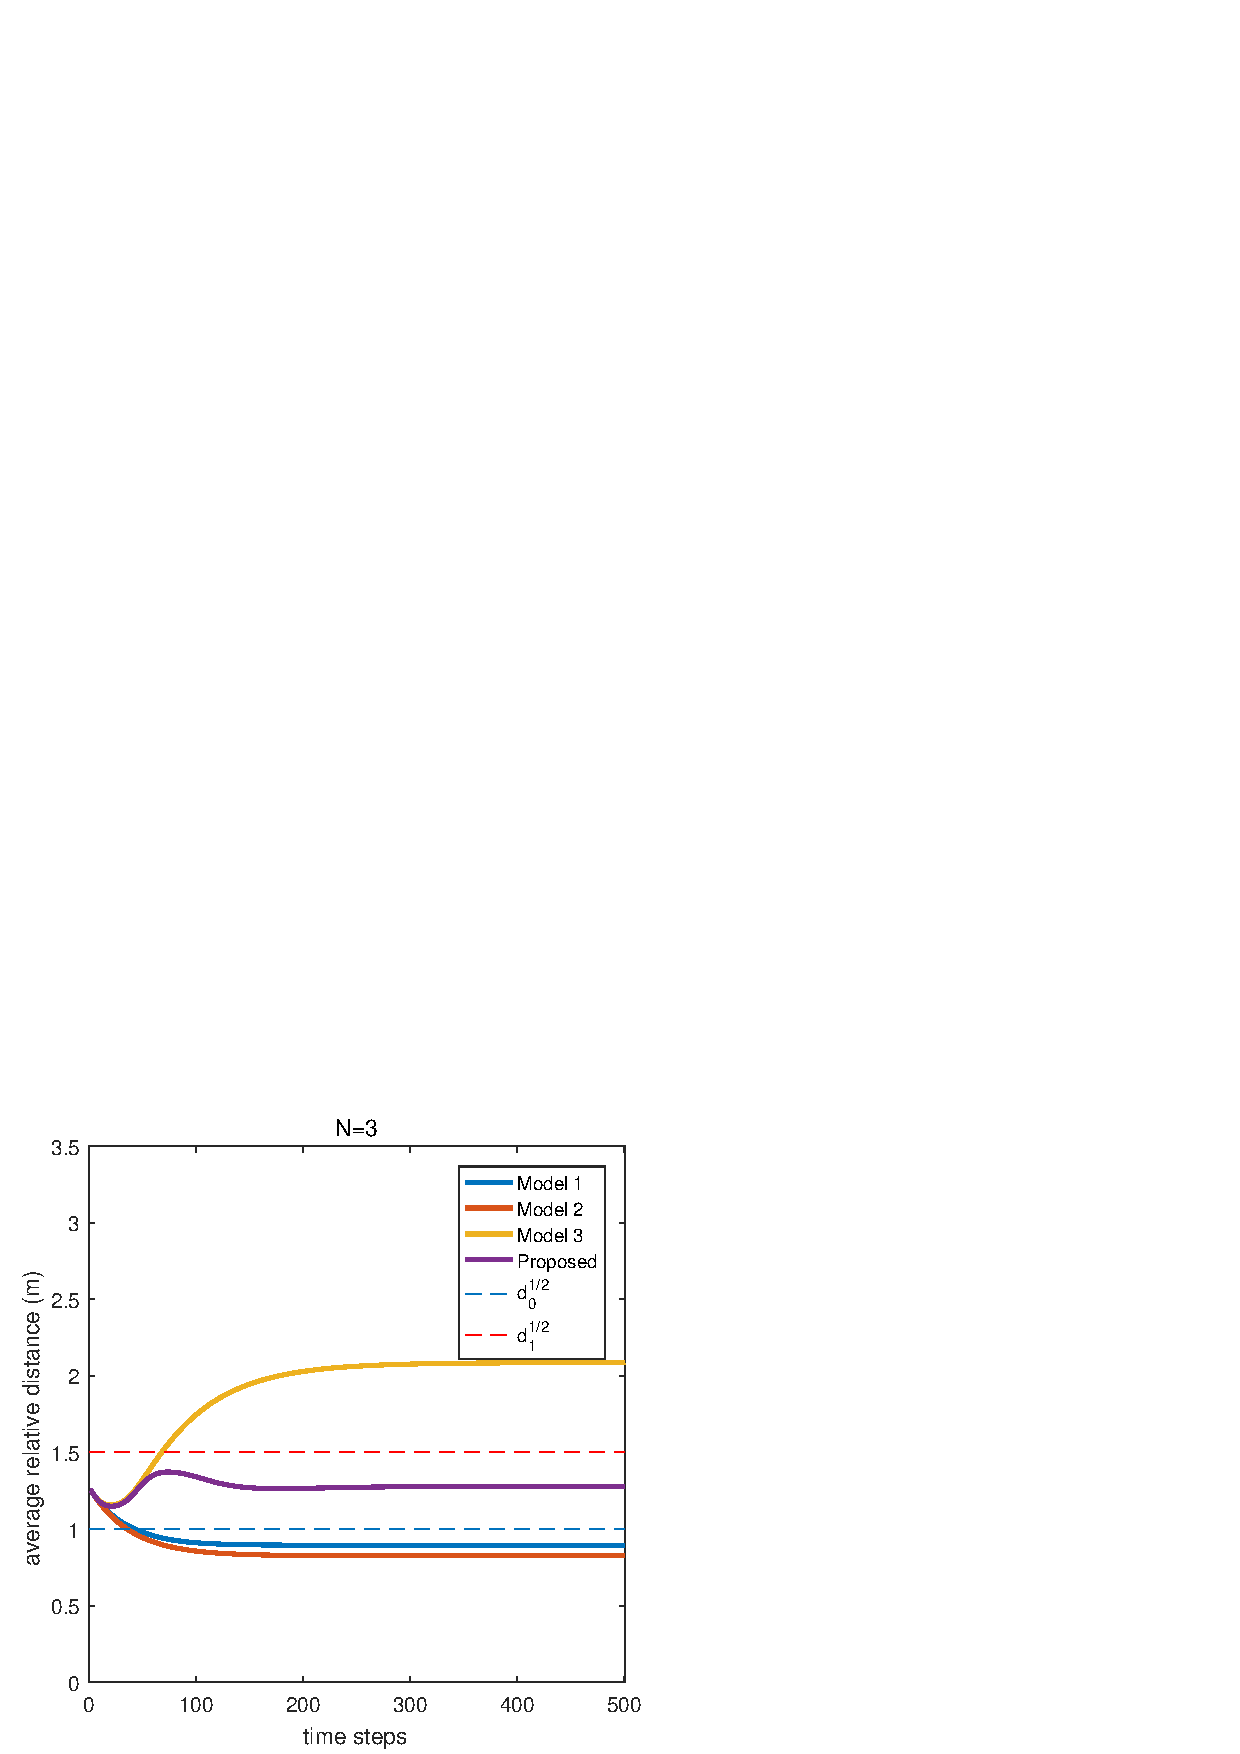
\includegraphics[width=0.49\textwidth]{figure/chapter_5/N3_dis.png}}
  \quad
  \subfigure[$N=4$ agents.]{\label{fig:N4_dis}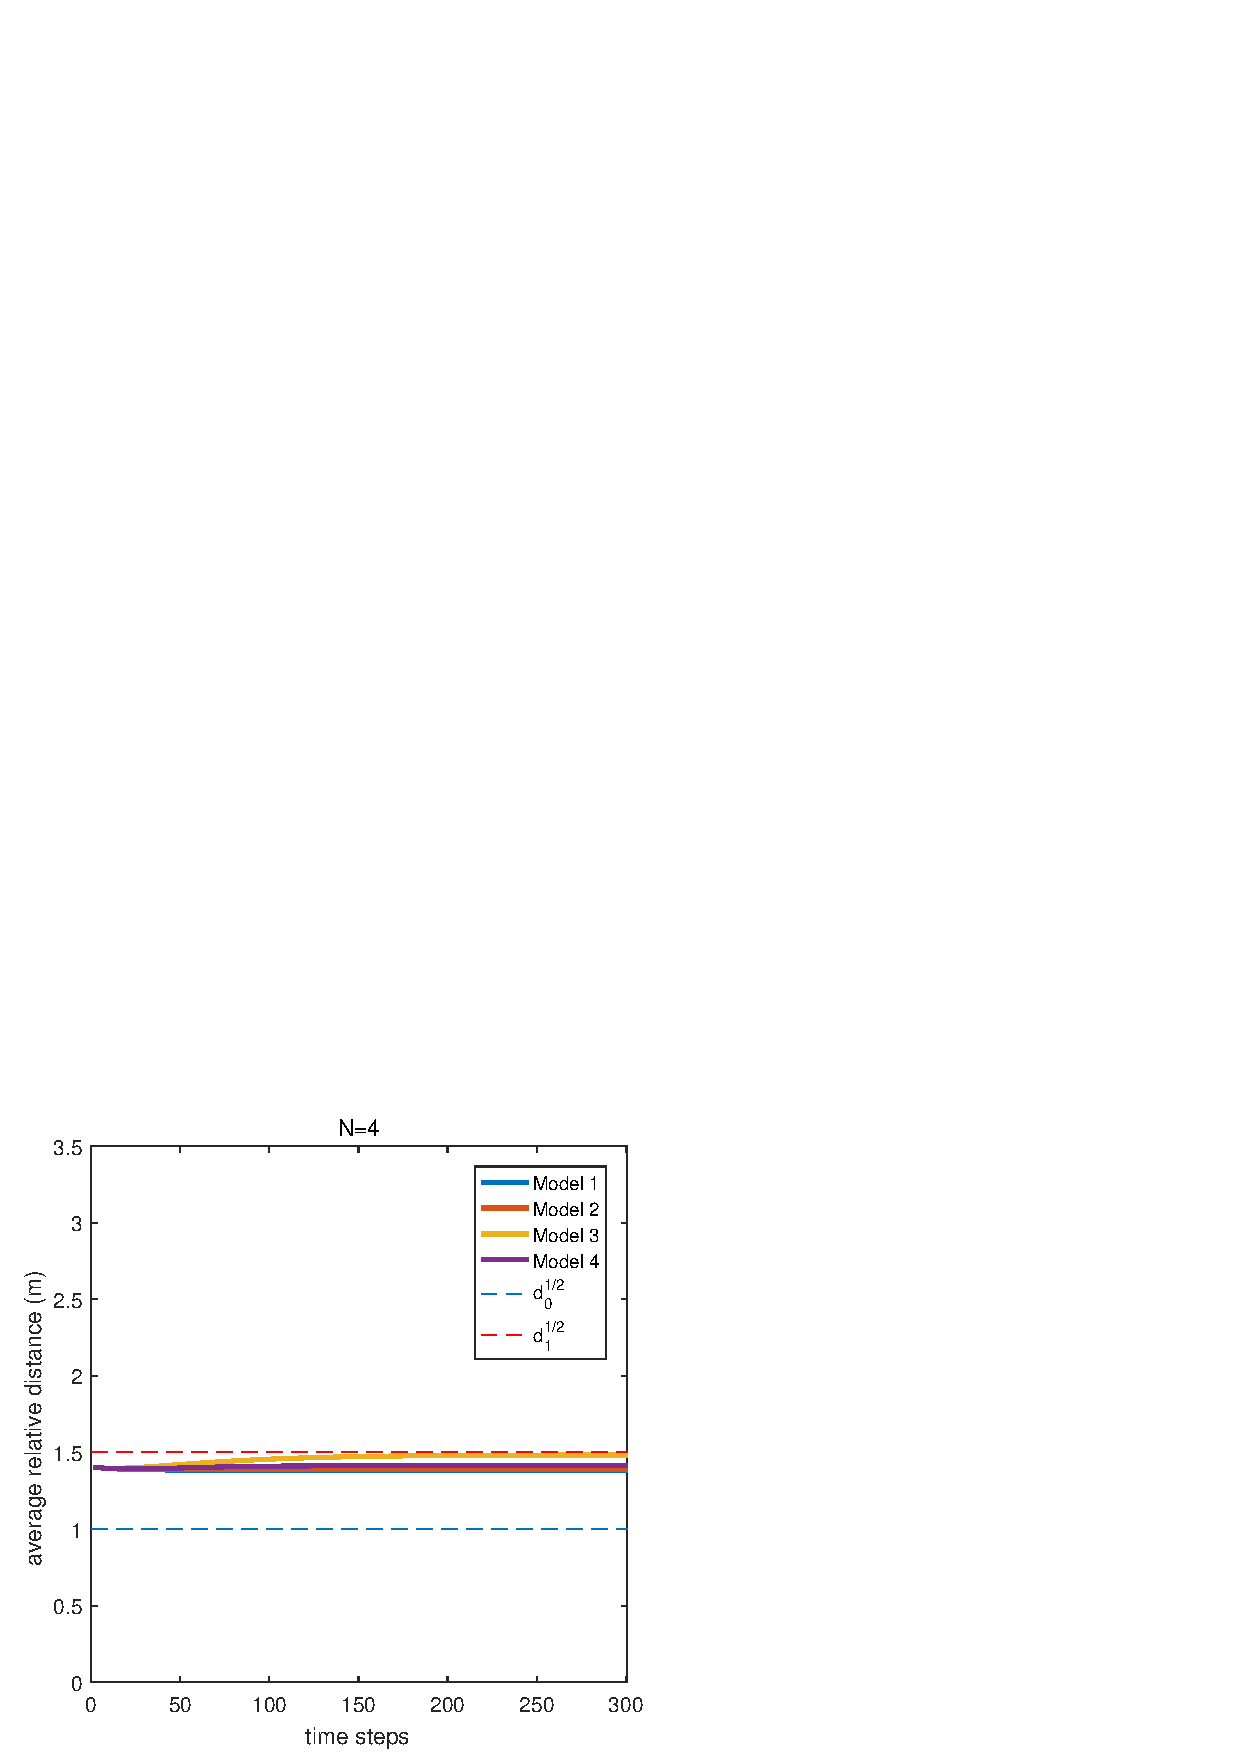
\includegraphics[width=0.49\textwidth]{figure/chapter_5/N4_dis.png}}
  \caption{Average relative distance between neighboring agents. The blue and red dashed line indicate two boundaries $d_0^{\frac{1}{2}}, d_1^{\frac{1}{2}}$ in our proposed model. Model 1, 2 and 3 are from~\cite{Vicsek1995},\cite{CuckerSmale2007} and \cite{CuckerDong2010} respectively.}\label{fig:N_dis}
\end{figure}

\begin{figure}[H]
  \centering
  \subfigure[$N=2$ agents.]{\label{fig:N2_pos}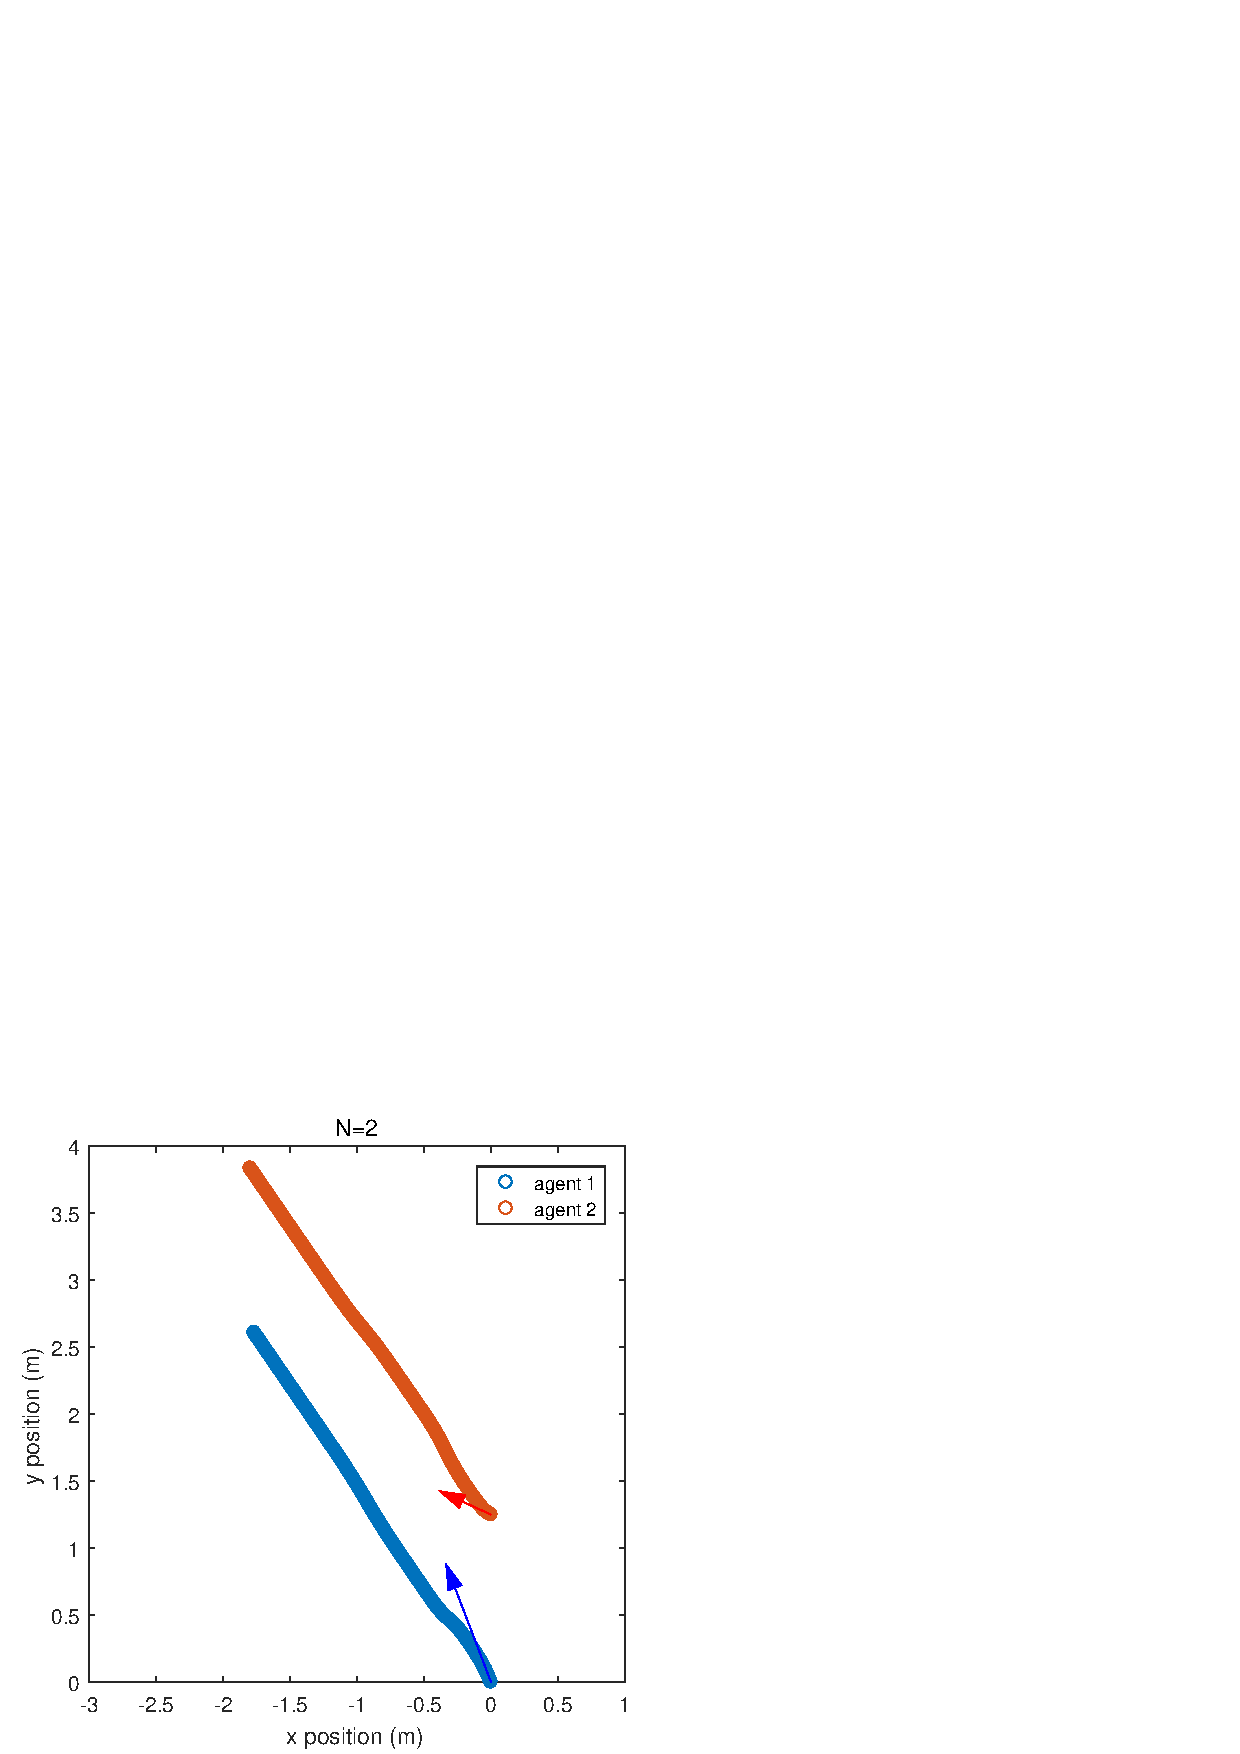
\includegraphics[width=0.49\textwidth]{figure/chapter_5/N2_pos.png}}
  \subfigure[$N=3$ agents.]{\label{fig:N3_pos}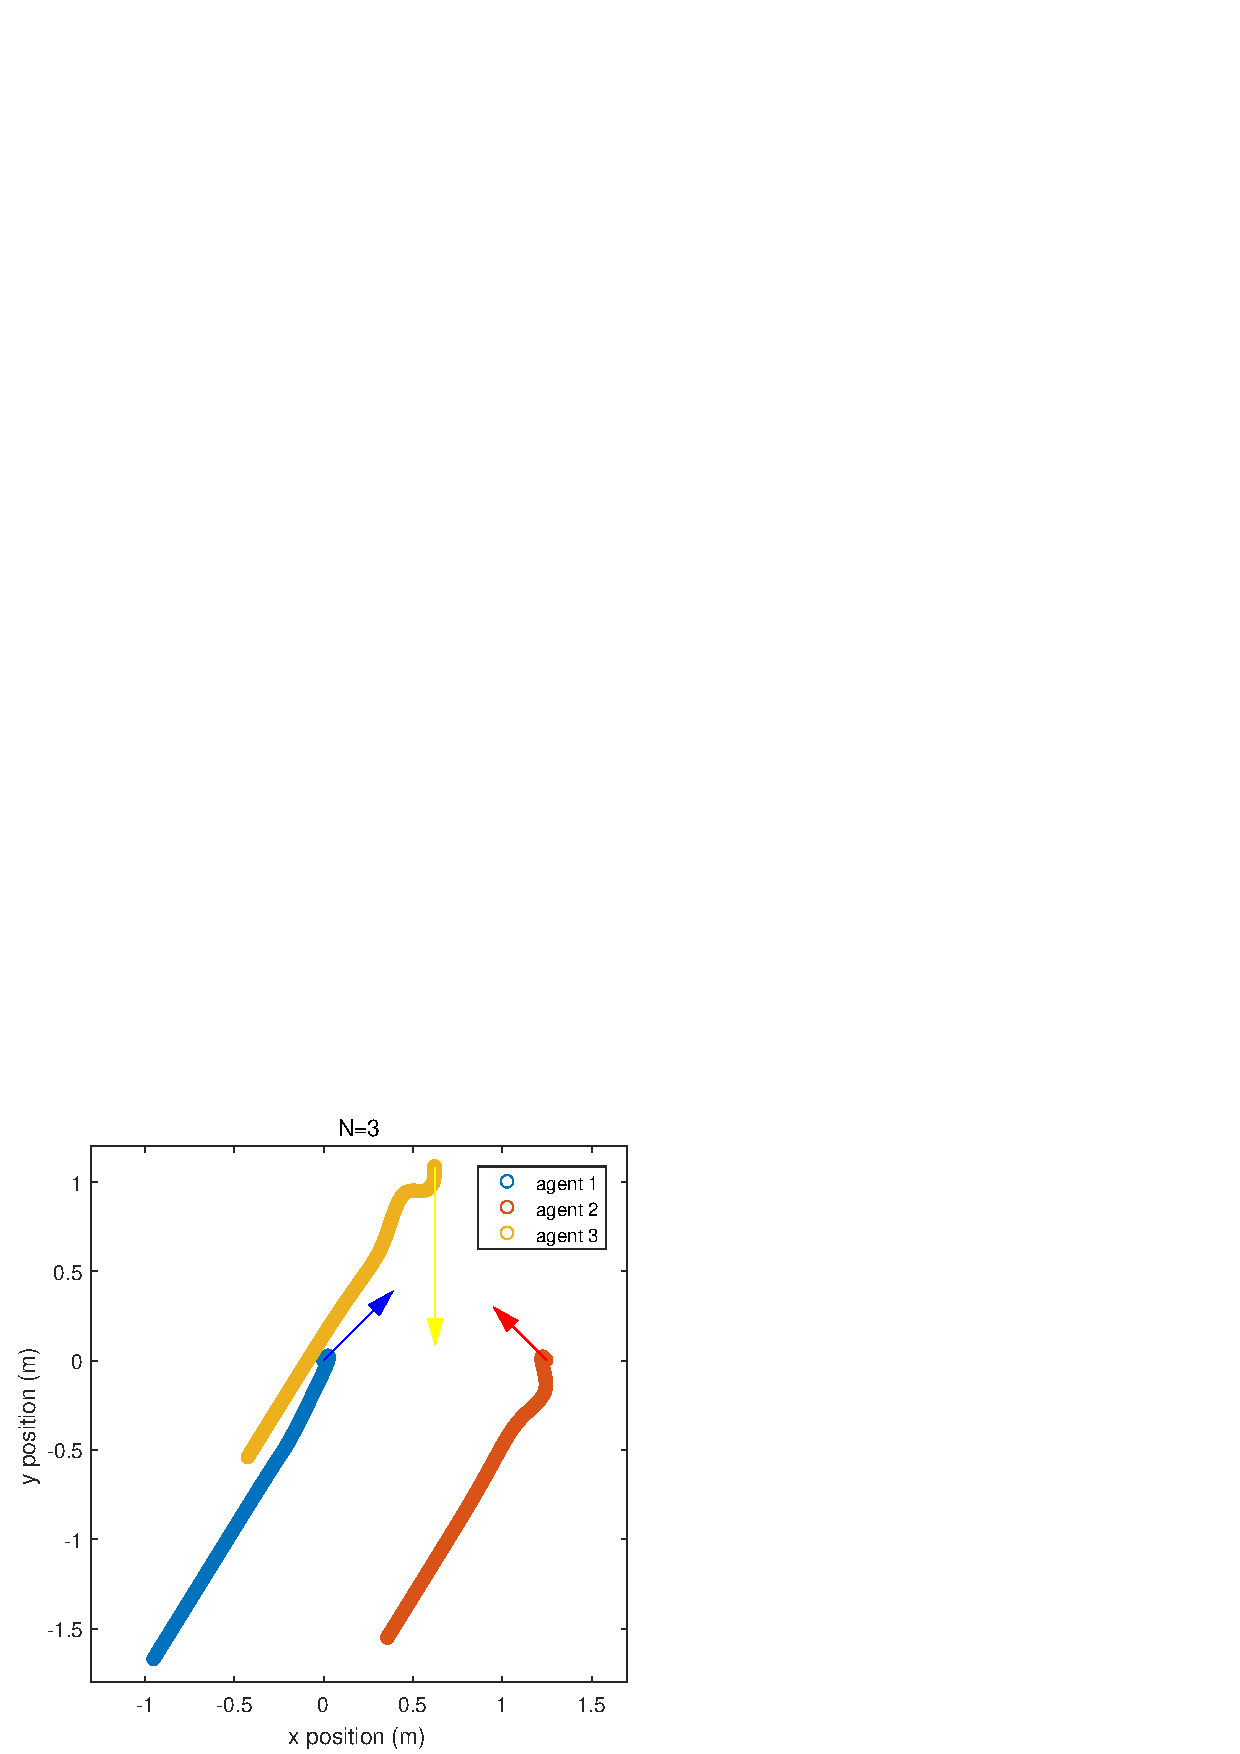
\includegraphics[width=0.49\textwidth]{figure/chapter_5/N3_pos.png}}
  \quad
  \subfigure[$N=4$ agents.]{\label{fig:N4_pos}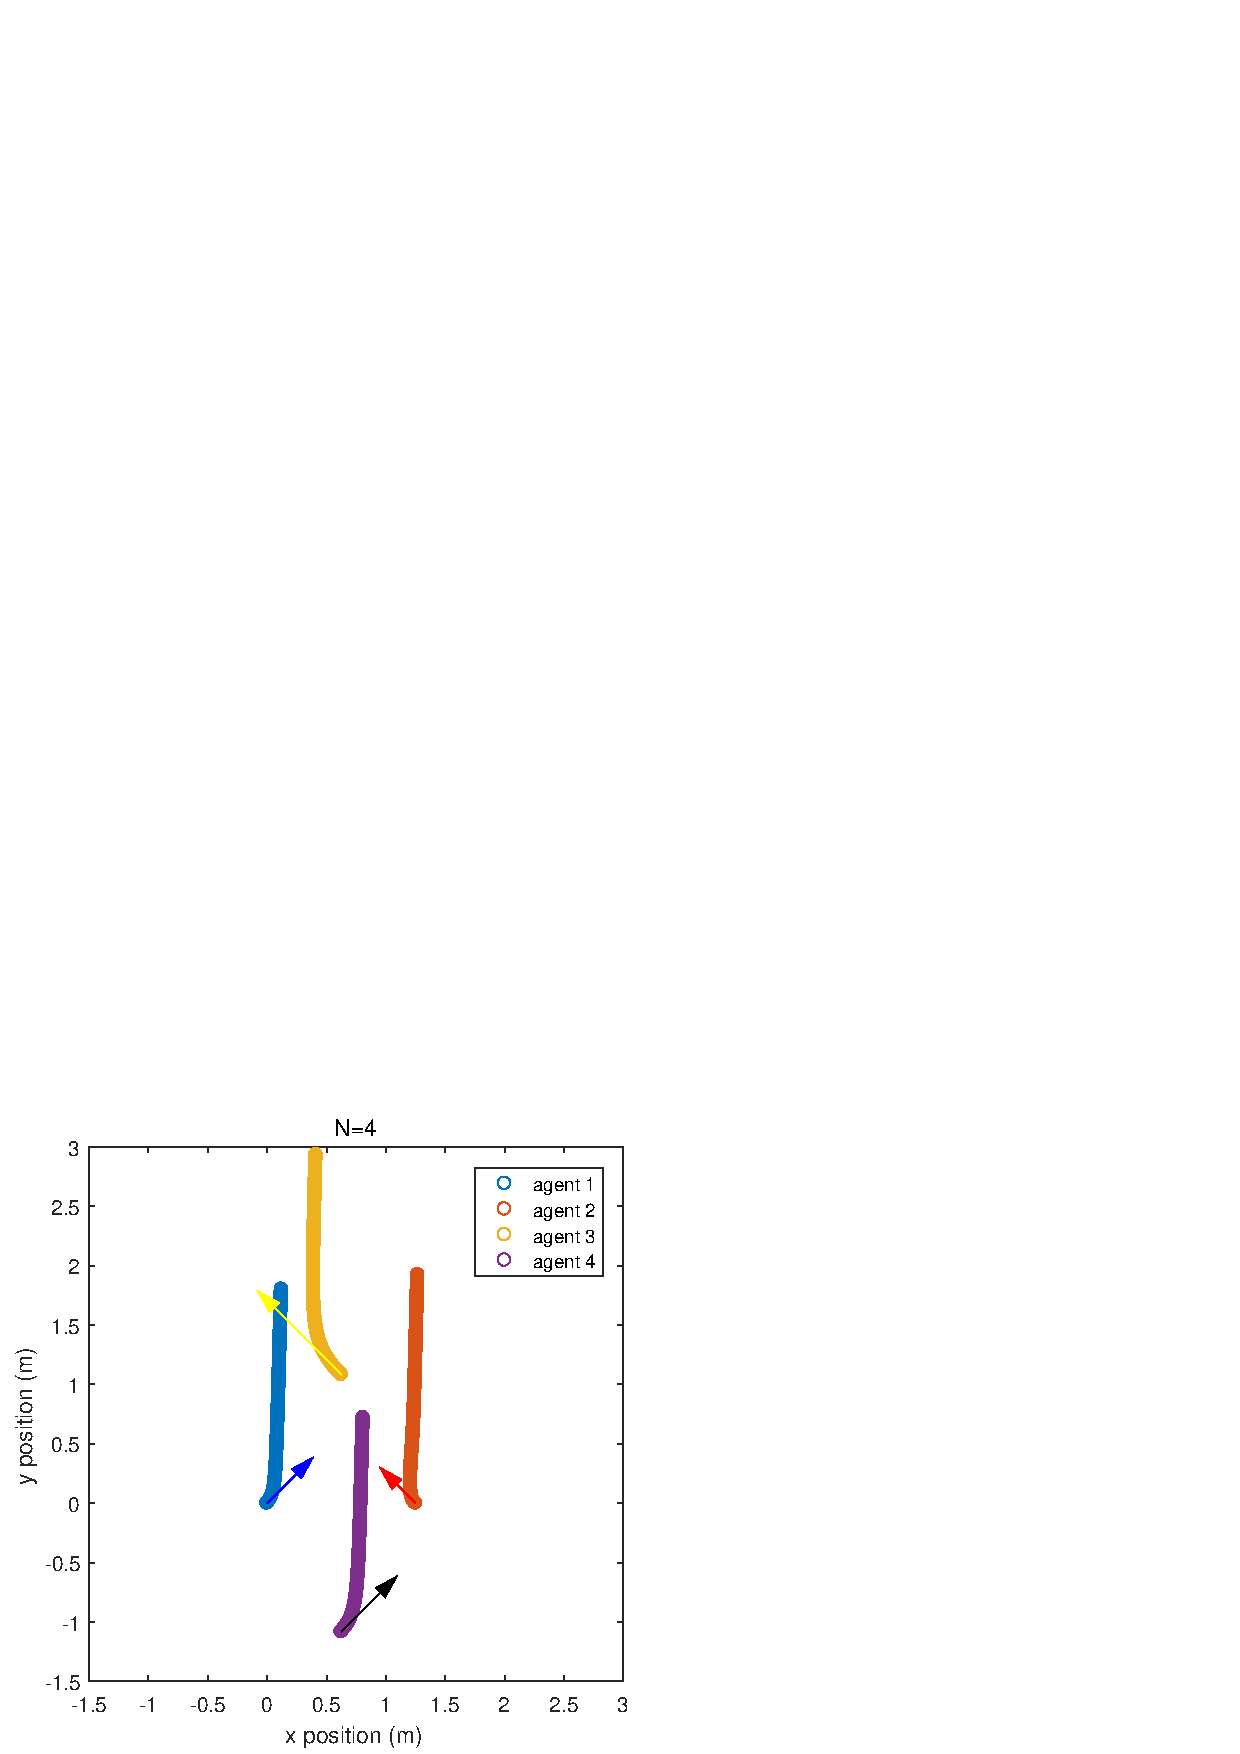
\includegraphics[width=0.49\textwidth]{figure/chapter_5/N4_pos.png}}
  \caption{Motion simulations with normalized initial velocities whose directions are indicated by corresponding arrows.}\label{fig:N_pos}
\end{figure}

\section{Comparison with Tracking Algorithm}\label{tracking}

We have compared the cohesion, separation and alignment performance from our proposed flocking model with those solved by the traditional tracking algorithm. Inspired by~\cite{Chenjing}, we develop a similar method for the chaser UAV to stay $d_s$ away from the target UAV. The entire procedure consists two parts: $\mathit{I}$, target UAV motion estimation and prediction and $\mathit{II}$, chaser UAV trajectory generation. In~\ref{fig:rviz}, the pink arrow (10Hz) indicates the heading of the target UAV and the dark green arrows (400Hz) are the poses of the follower UAV. The light green dots are the 3D positions of the target calculated from captured images, a frame of which is shown in Fig.\ref{fig:capture}. The blue curve and the red one are the predicted path and generated trajectory respectively. As illustrated in Fig.\ref{fig:track_plot}, the developed algorithm has successfully driven the chaser UAV to track the target UAV, however, it is clearly seen in Fig.\ref{fig:position_plot} that the delay is inevitable.

\begin{figure}[htb]
  \centering
  \subfigure[Target motion estimation, prediction and chaser trajectory generation visualized on rviz with data from rosbag.]{\label{fig:rviz}\includegraphics[width=0.49\textwidth]{figure/chapter_5/rviz.png}}
  \subfigure[Image captured from chaser's on-board camera. Green square indicates the recognized aruco code carried on target's UAV.]{\label{fig:capture}\includegraphics[width=0.49\textwidth]{figure/chapter_5/capture.png}}
  \caption{Screenshots of the tracking algorithm.}\label{fig:rviz_capture}
\end{figure}

\subsection{Target Motion Estimation and Prediction}

We denote the 3D position of the target at time t $\in \mathbb{R}$ as T(t) $\in \mathbb{R}^{3}$ and expand it with Taylor Series. We omit the high order terms $(n>5)$ and approximate it with the $5^{th}$ order polynomial $\hat{T}(t) \in \mathbb{R}^{3}$:

\begin{equation}\label{eq:poly5}
T(t) = \sum^n_{i=0} a_{i}t^i
\approx \sum^5_{i=0} a_{i}t^i
= \begin{bmatrix}1\\t\\t^2\\t^3\\t^4\\t^5\end{bmatrix}^T\begin{bmatrix}a_0\\a_1\\a_2\\a_3\\a_4\\a_5\end{bmatrix}
= T^TA = \hat{T}(t)
\end{equation}

\noindent
Assuming the target's motion is smooth and continuous, we add acceleration regulator $\lambda_{t}$ and minimize the following:

\begin{equation}\label{eq:minT}
\min_{\hat{T}(\cdot)} \sum^{L}_{i=0} ||\hat{T}(t_i)-p_i||^2_2 + \lambda_t\int_{t_l}^{t_m} ||\hat{T}^{(2)}(t)||^2_2dt
\end{equation}

\noindent
where $L$ is the total number of observations captured and $p_i$ is the $i^{th}$ target position in global frame at time $t_i$. Note here that $[t_l, t_0]$ is the time period we actually have target observations and $[t_0, t_m]$ is the period we make predictions for target's motion (\ref{eq:minF}).


\subsection{Trajectory Generation}

During the tracking task, the chaser UAV is expected to keep a fixed distance $d_s\in\mathbb{R}^{3}$ from the target. In this scenario, the chaser UAV is supposed to follow the shifted predicted target trajectory $T_s(t)=\hat{T}(t)+d_s$. Similarly, we denote the planned trajectory for chaser UAV with $f(t)=\sum^5_{i=0} e_{i}t^i=T^TE$ and adjust the tracking stiffness with regulator $\lambda_f$. We then minimize the following:

\begin{equation}\label{eq:minF}
\begin{aligned}
&\min_{f(\cdot)} \int_{t_0}^{t_m} ||f(t)-T_s(t)||^2_{2}dt + \lambda_f\int_{t_0}^{t_m} ||f^{(3)}(t)||^2_{2}dt\\
&s.t.
\end{aligned}
\end{equation}

\begin{equation}
\underbrace{f(t_0)=f_0}_{\text{initial state constraint}}
\end{equation}

\begin{equation}
\underbrace{f(t_m)=0}_{\text{ending state constraint}}
\end{equation}

\begin{equation}
\underbrace{f^{(1)}(t) \in \Omega_{v}(t)}_{\text{velocity constraint}}
\end{equation}

\begin{equation}
\underbrace{f^{(2)}(t) \in \Omega_{a}(t)}_{\text{acceleration constraint}}
\end{equation}

\noindent
where $f_0$ is the state of the chaser UAV at the beginning of the trajectory and $\Omega_v$ and $\Omega_a$ are the velocity and acceleration constraints respectively.

We can rewrite (\ref{eq:minF}) as:

\begin{equation}\label{eq:reminF1}
\min_{l\in\{x,y,z\}}\int_{0}^{t_m-t_0} (A^TT_sT_s^TA-2E^TT^TT_s^TA+E^TT^TTE)dt + \lambda_f\int_{0}^{t_m-t_0} (E^TT_fT_f^TE)dt\\
\end{equation}

\noindent
and transform (\ref{eq:reminF1}) into a standard QP problem:

\begin{equation}\label{eq:reminF2}
\min_{l\in\{x,y,z\}}E^T[\int_{0}^{t_m-t_0}(T^TT+T_fT_f^T)dt]E-2E^T[\int_{0}^{t_m-t_0}T_f^TT_s^T]A
\end{equation}

\noindent
where $T_s = \begin{bmatrix}1\\1+dT\\(1+dT)^2\\(1+dT)^3\\(1+dT)^4\\(1+dT)^5\end{bmatrix}$ and $T_f=\begin{bmatrix}0\\0\\0\\6\\24t\\60t^2\end{bmatrix}$ with $dT=t_0-t_l$. We use $l\in\{x,y,z\}$ to abstract the dimension.

\subsection{Tracking Performance}

\begin{figure}[H]
  \centering
  \subfigure[Position profiles of target and chaser UAVs. The blue and red lines are the x and y positions of the target UAV and the yellow and the purple lines are the x and y positions of the chaser UAV.]{\label{fig:position_plot}\includegraphics[width=0.49\textwidth]{figure/chapter_5/position_plot.png}}
  \subfigure[Relative distance between target and chaser UAVs. The desired shifted distance $d_s=1.5$ while the averaged relative distance $\bar{d}=1.39$.]{\label{fig:distance_plot}\includegraphics[width=0.49\textwidth]{figure/chapter_5/distance_plot.png}}
  \quad
  \subfigure[$\psi_{scal}$ of the tracking system.]{\label{fig:scal_plot}\includegraphics[width=0.49\textwidth]{figure/chapter_5/scal_plot.png}}
  \subfigure[\textcolor{red}{rviz}]{\label{fig:rviz_plot}\includegraphics[width=0.49\textwidth]{figure/chapter_5/scal_plot.png}}
  \caption{\textcolor{red}{TODO: Modify $\psi_{scal}$ plot.}}\label{fig:track_plot}
\end{figure}

\section{Realization of Proposed Model}

In this section, we demonstrate that our flocking system is able to manipulate in both indoor GPS-denied and outdoor natural environment. All the experiment settings are identical, where the follower UAV takes off first and hovers at desired height, waiting for the leader, then the leader UAV takes off and the control authority of follower switches to autonomous mode to begin flocking. The initial take off position of follower UAV is 1.5 m behind the leader UAV to match the requirement ($d_0<||x_i-x_j||^2<d_1$) in Ch.\ref{control_law}. The maximum acceleration and velocity of follower UAV are set to $a_{max}=2.5 m/s^2$ and $v_{max}=0.5 m/s$ for safety reasons. In each experiment we show their position profile, relative distance, $\psi_{scal}$ plot and their movement path reproduced in rivz. Due to measurement noise and lack of ground truth, spikes appear randomly in all figures. The trend of slope in $\psi_{cal}$ plot, however, is in accordance with that in position plot.

\subsection{Indoor Environment}

We first show the results when the leader UAV moves purely in the directions of x-axis and y-axis as illustrated in Fig.\ref{fig:x_indoor} and Fig.\ref{fig:y_indoor}.

\begin{figure}[htb]
  \centering
  \subfigure[Position profiles of leader and follower UAVs. The yellow and purple lines are the x and y positions of the leader UAV and the blue and the red lines are the x and y positions of the follower UAV.]{\label{fig:x_indoor_position}\includegraphics[width=0.49\textwidth]{figure/chapter_5/x_indoor_position.png}}
  \subfigure[Relative distance between leader and follower UAVs.]{\label{fig:x_indoor_distance}\includegraphics[width=0.49\textwidth]{figure/chapter_5/x_indoor_distance.png}}
  \quad
  \subfigure[$\psi_{scal}$]{\label{fig:x_indoor_scal}\includegraphics[width=0.49\textwidth]{figure/chapter_5/x_indoor_scal.png}}
  \subfigure[\textcolor{red}{rviz}]{\label{fig:x_indoor_rviz}\includegraphics[width=0.49\textwidth]{figure/chapter_5/x_indoor_scal.png}}
  \caption{Flocking in x-axis.}\label{fig:x_indoor}
\end{figure}

\begin{figure}[htb]
  \centering
  \subfigure[Position profiles of leader and follower UAVs. The yellow and purple lines are the x and y positions of the leader UAV and the blue and the red lines are the x and y positions of the follower UAV.]{\label{fig:y_indoor_position}\includegraphics[width=0.49\textwidth]{figure/chapter_5/y_indoor_position.png}}
  \subfigure[Relative distance between leader and follower UAVs.]{\label{fig:y_indoor_distance}\includegraphics[width=0.49\textwidth]{figure/chapter_5/y_indoor_distance.png}}
  \quad
  \subfigure[$\psi_{scal}$]{\label{fig:y_indoor_scal}\includegraphics[width=0.49\textwidth]{figure/chapter_5/y_indoor_scal.png}}
  \subfigure[\textcolor{red}{rviz}]{\label{fig:y_indoor_rviz}\includegraphics[width=0.49\textwidth]{figure/chapter_5/y_indoor_scal.png}}
  \caption{Flocking in y-axis.}\label{fig:y_indoor}
\end{figure}

\subsection{Outdoor Environment}

We first show the results when leader UAV moves purely in the directions of x-axis and y-axis as illustrated in Fig.\ref{fig:x_indoor} and Fig.\ref{fig:y_indoor}. The follower UAV could keep moving with the leader UAV, however, due to the measurement noise and the limitation of maximum acceleration of follower UAV, the relative distance and $\psi_{scal}$ have spikes.

\begin{figure}[htb]
  \centering
  \subfigure[Position profiles of leader and follower UAVs. The yellow and purple lines are the x and y positions of the leader UAV and the blue and the red lines are the x and y positions of the follower UAV.]{\label{fig:xy_outdoor_position}\includegraphics[width=0.49\textwidth]{figure/chapter_5/xy_outdoor_position.png}}
  \subfigure[Relative distance between leader and follower UAVs.]{\label{fig:xy_outdoor_distance}\includegraphics[width=0.49\textwidth]{figure/chapter_5/xy_outdoor_distance.png}}
  \quad
  \subfigure[$\psi_{scal}$]{\label{fig:xy_outdoor_scal}\includegraphics[width=0.49\textwidth]{figure/chapter_5/xy_outdoor_scal.png}}
  \subfigure[\textcolor{red}{rviz}]{\label{fig:xy_outdoor_rviz}\includegraphics[width=0.49\textwidth]{figure/chapter_5/y_indoor_scal.png}}
  \caption{Flocking in xy-plane.}\label{fig:xy_outdoor}
\end{figure}

\newpage
